%%%%%%%%%%%%%%%%%%%%%%%%%%%%%%%%%%%%%%%%%%%%%%%%%%%%%%%%%%%%%%%%%%% 
%         Template for a short thesis all in one file             %
%        (titlepage info below assumes masters degree}            %
%  Just run latex (or pdflatex) on this file to see how it looks  %
%      Be sure to run twice to get correct TOC and citations      %
%%%%%%%%%%%%%%%%%%%%%%%%%%%%%%%%%%%%%%%%%%%%%%%%%%%%%%%%%%%%%%%%%%% 
%
%  To produce the abstract title page followed by the abstract,
%  see the template file, "abstitle-mas.tex"
%
%%%%%%%%%%%%%%%%%%%%%%%%%%%%%%%%%%%%%%%%%%%%%%%%%%%%%%%%%%%%%%%%%%%

\documentclass{thesis}
\usepackage{graphicx}   % if you want to include graphics files


% Bibliography
% As per VU requirements, references must be in alphabetical order, so we use sorting=nyt (name, year, title).
\RequirePackage[style=nature,sorting=nyt,natbib=true,backend=biber]{biblatex}
\addbibresource{references.bib}

% Add biblography hyperref
\usepackage{hyperref}


% Use booktabs
\usepackage{booktabs}


% Use the first command below if you want captions over 1 line indented.
% A side effect of this is to remove the use of bold for captions. 
% To restore bold, also include the second line below.
%\usepackage[hang]{caption}     % to indent subsequent lines of captions
%\renewcommand{\captionfont}{\bfseries} % only needed with caption package;
                                        %   otherwise bold is default)
                                        
%%%%%%%%%%%%%%%%%%%%  supply titlepage info  %%%%%%%%%%%%%%%%%%%%%
\thesistitle{\bf Differential Equations\\On two lines}     % Your thesis title
\author{Sir Isaac Newton}   % Your full name
\degree{Master of Science}  % Master of Science, Doctor of Philosophy, ...
\programname{Computer Science}  % name of your program: E.g.: Computer Science, Biology, Software Engineering,...
\department{Computing Sciences} % provide your area of study here; e.g.,
\thadviser{Galileo Galilei}  % The full name of your advisor
%\cothadviser{First co-adviser} %if needed
%\cocothadviser{Second co-adviser} % if needed
%  For a masters project use \projadviser instead of \thadviser, 
%  and \coprojadviser and \cocoprojadviser if needed. 
\submitdate{January, 1685}        
%\copyrightyear{1685}  % if date omitted, current year is used. 
%%%%%%%%%%%%%%%%%%%%%   end titlepage info  %%%%%%%%%%%%%%%%%%%%%%
      
\begin{document} 
\titlepage             % Print titlepage   
%\copyrightpage        % optional         
\tableofcontents       % required 
\listoftables          % required if there are tables
\listoffigures         % required if there are figures

\specialhead{ACKNOWLEDGMENT}
The acknowledgment text goes here. Unlike chapter headings, 
this heading is not numbered.

\specialhead{ABSTRACT}
An abstract (limited to 150 words for Master’s Thesis and 350 words for Doctoral
Dissertation) must be prepared on a single page.

\chapter{Introduction}


The text of the first chapter goes here. To cite a reference for the
bibliography, use a command such as: \cite{newton1934principia} (normal citation) and like \citet{einstein1916foundation} (textual citation) did.
\section{A Section Heading}
This is a sentence to take up space and look like text.
\subsection{A Subsection Heading}


\chapter{Another Chapter}

This is another chapter and it has a table. You can reference Table \ref{tab:a_table} using the command \ref{tab:a_table}.

\section{Tables}

\begin{table}[ht]
    \centering
    \begin{tabular}{cc}
         \textbf{X} & \textbf{Y}  \\ \toprule
         1 & 2 \\
         1 & 2 \\
         1 & 2 \\ \bottomrule
    \end{tabular}
    \caption{This is a table.}
    \label{tab:a_table}
\end{table}


\section{Figures}

This chapter also has a figure (see Figure \ref{fig:a_figure}).

\begin{figure}[ht]
    \centering
    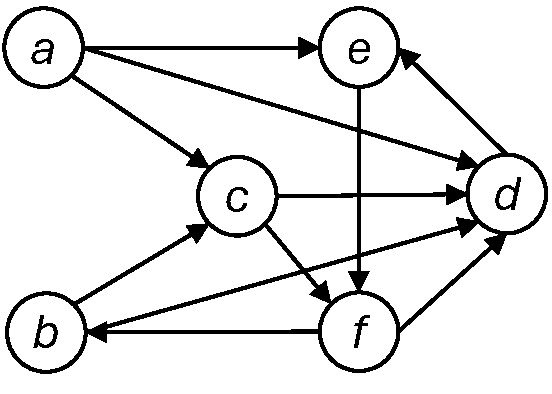
\includegraphics[width=0.5\linewidth]{figures/g1.pdf}
    \caption{A figure showing a directed graph. Prefer vectorized formats like PDF and EPS instead of JPG and PNG.}
    \label{fig:a_figure}
\end{figure}


% The following produces a numbered bibliography where the numbers
% correspond to the \cite commands in the text.
% \specialhead{LITERATURE CITED}


\begin{singlespace}
\printbibliography
\end{singlespace}

%%%%%%%%%%%%%%%%%%%%%%%  For Appendices  %%%%%%%%%%%%%%%%%%%
\appendix    % This command is used only once!
\addtocontents{toc}{\parindent0pt\vskip12pt APPENDICES} %toc entry, no page #


\chapter{First Appendix}
Note the numbering of the chapter heading is changed.
This is a sentence to take up space and look like text.
\section{A Section Heading}
This is how equations are numbered in an appendix:
\begin{equation}
x^2 + y^2 = z^2
\end{equation} 
\chapter{Second Appendix}
This is a sentence to take up space and look like text.



\end{document}
